% answers.tex —— 1995 年·全国卷·文科 · 参考答案与详细解析片段
% 由 tools/generate_projects.py 依来源总账自 1995/1995_数学真题_全国文_试题.md + 1995/1995_数学真题_全国文_解析正文.md + 1995/1995_数学真题_全国文_答案要点.md 生成，勿手改（改源 MD 后重跑）


\begin{answer}
\gksolhead{1}{}

\textbf{题目}：

已知集合 $I=\{0,-1,-2,-3,-4\}$，集合 $M=\{0,-1,-2\}$，$N=\{0,-3,-4\}$，则 $\overline{M}\cap N=$\mbox{（　　）}。

（A）$\{0\}$　　（B）$\{-3,-4\}$　　（C）$\{-1,-2\}$　　（D）$\varnothing$

\Needspace{4\baselineskip}
\textbf{解析}

在全集 $I$ 内取 $M$ 的补集：$\complement_I M=I\setminus M=\{-3,-4\}$；再与 $N=\{0,-3,-4\}$ 取交集，得 $\{-3,-4\}$。

\gkanswer{答案：B。}

\end{answer}
\begin{answer}
\gksolhead{2}{}

\textbf{题目}：

函数 $y=\dfrac{1}{x+1}$ 的图象是\mbox{（　　）}。
\nopagebreak[4]
\begin{center}% 固定来源PDF印刷页52第2题四个图象选项的矢量示意重绘。
% 渐近线位置、分支所在象限及选项标签忠于原页；比例仅作示意。
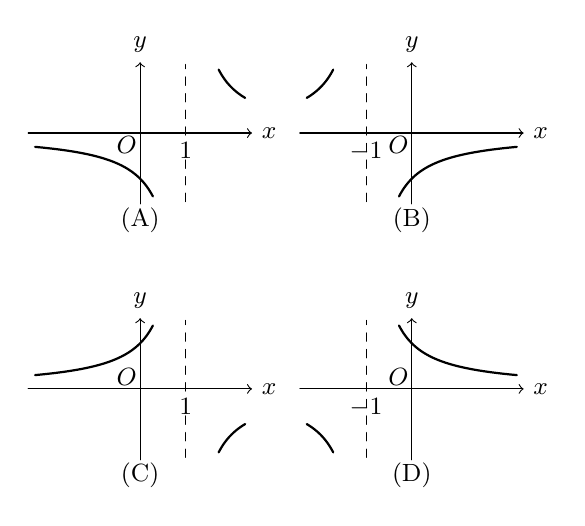
\begin{tikzpicture}[x=.58cm,y=.58cm,font=\small,line cap=round,line join=round]
  % (A) y=1/(x-1)
  \begin{scope}
    \draw[->] (-2.45,0)--(2.45,0) node[right] {$x$};
    \draw[->] (0,-1.55)--(0,1.55) node[above] {$y$};
    \draw[dashed] (1,-1.5)--(1,1.5);
    \draw[thick,domain=-2.3:.28,samples=60,variable=\x] plot (\x,{1/(\x-1)});
    \draw[thick,domain=1.72:2.3,samples=60,variable=\x] plot (\x,{1/(\x-1)});
    \node[below] at (1,0) {$1$};
    \node[below left,inner sep=1pt] at (0,0) {$O$};
    \node at (0,-1.9) {(A)};
  \end{scope}

  % (B) y=-1/(x+1)
  \begin{scope}[xshift=3.45cm]
    \draw[->] (-2.45,0)--(2.45,0) node[right] {$x$};
    \draw[->] (0,-1.55)--(0,1.55) node[above] {$y$};
    \draw[dashed] (-1,-1.5)--(-1,1.5);
    \draw[thick,domain=-2.3:-1.72,samples=60,variable=\x] plot (\x,{-1/(\x+1)});
    \draw[thick,domain=-.28:2.3,samples=60,variable=\x] plot (\x,{-1/(\x+1)});
    \node[below] at (-1,0) {$-1$};
    \node[below left,inner sep=1pt] at (0,0) {$O$};
    \node at (0,-1.9) {(B)};
  \end{scope}

  % (C) y=-1/(x-1)
  \begin{scope}[yshift=-3.25cm]
    \draw[->] (-2.45,0)--(2.45,0) node[right] {$x$};
    \draw[->] (0,-1.55)--(0,1.55) node[above] {$y$};
    \draw[dashed] (1,-1.5)--(1,1.5);
    \draw[thick,domain=-2.3:.28,samples=60,variable=\x] plot (\x,{-1/(\x-1)});
    \draw[thick,domain=1.72:2.3,samples=60,variable=\x] plot (\x,{-1/(\x-1)});
    \node[below] at (1,0) {$1$};
    \node[above left,inner sep=1pt] at (0,0) {$O$};
    \node at (0,-1.9) {(C)};
  \end{scope}

  % (D) y=1/(x+1), the graph of the stated function.
  \begin{scope}[xshift=3.45cm,yshift=-3.25cm]
    \draw[->] (-2.45,0)--(2.45,0) node[right] {$x$};
    \draw[->] (0,-1.55)--(0,1.55) node[above] {$y$};
    \draw[dashed] (-1,-1.5)--(-1,1.5);
    \draw[thick,domain=-2.3:-1.72,samples=60,variable=\x] plot (\x,{1/(\x+1)});
    \draw[thick,domain=-.28:2.3,samples=60,variable=\x] plot (\x,{1/(\x+1)});
    \node[below] at (-1,0) {$-1$};
    \node[above left,inner sep=1pt] at (0,0) {$O$};
    \node at (0,-1.9) {(D)};
  \end{scope}
\end{tikzpicture}
\end{center}
\nopagebreak[4]
\Needspace{4\baselineskip}
\textbf{解析}

$y=\dfrac{1}{x+1}$ 的定义域为 $x\ne-1$，竖直渐近线 $x=-1$，水平渐近线 $y=0$；且 $x>-1$ 时 $y>0$（右支在 $x$ 轴上方），$x<-1$ 时 $y<0$（左支在 $x$ 轴下方）。逐图核对：(A) 渐近线为 $x=1$；(B) 渐近线为 $x=-1$ 但两支符号与 $y=\dfrac1{x+1}$ 相反（右支在下、左支在上）；(C) 渐近线为 $x=1$ 且两支符号相反；(D) 渐近线 $x=-1$，右支在上、左支在下，与所给函数一致。

\gkanswer{答案：D。}

\end{answer}
\begin{answer}
\gksolhead{3}{}

\textbf{题目}：

\Needspace{5\baselineskip}
函数
\nopagebreak[4]
\[
y=4\sin\left(3x+\frac\pi4\right)+3\cos\left(3x+\frac\pi4\right)
\]
的最小正周期是\mbox{（　　）}。

（A）$6\pi$　　（B）$2\pi$　　（C）$\dfrac{2\pi}{3}$　　（D）$\dfrac\pi3$

\Needspace{4\baselineskip}
\textbf{解析}

$4\sin u+3\cos u=5\sin(u+\varphi)$（$\cos\varphi=\tfrac45,\ \sin\varphi=\tfrac35$）。取 $u=3x+\dfrac\pi4$，则 $y=5\sin\!\left(3x+\dfrac\pi4+\varphi\right)$，其最小正周期为 $\dfrac{2\pi}{3}$。

\gkanswer{答案：C。}

\end{answer}
\begin{answer}
\gksolhead{4}{}

\textbf{题目}：

正方体的全面积是 $a^2$，它的顶点都在球面上，这个球的表面积是\mbox{（　　）}。

（A）$\dfrac{\pi a^2}{3}$　　（B）$\dfrac{\pi a^2}{2}$　　（C）$2\pi a^2$　　（D）$3\pi a^2$

\Needspace{4\baselineskip}
\textbf{解析}

设正方体棱长为 $s$，全面积 $6s^2=a^2$，故 $s=\dfrac{a}{\sqrt6}$。正方体的体对角线为其外接球直径，长 $s\sqrt3=\dfrac{a}{\sqrt2}$，于是球半径 $R=\dfrac{a}{2\sqrt2}$。球表面积 $S=4\pi R^2=4\pi\cdot\dfrac{a^2}{8}=\dfrac{\pi a^2}{2}$。

\gkanswer{答案：B。}

\end{answer}
\begin{answer}
\gksolhead{5}{}

\textbf{题目}：

如图，若图中的直线 $l_1,l_2,l_3$ 的斜率分别为 $k_1,k_2,k_3$，则\mbox{（　　）}。
\nopagebreak[4]
\begin{center}% 固定来源PDF印刷页52第5题三条直线斜率关系的矢量示意重绘。
% 仅表达斜率的正负与大小次序，不表示题设给定的精确坐标。
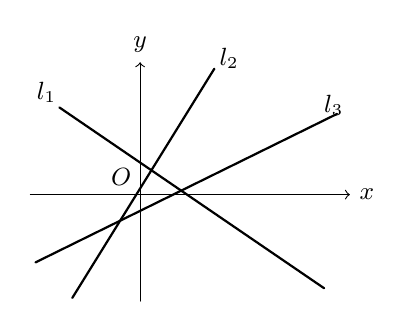
\begin{tikzpicture}[x=.82cm,y=.82cm,font=\small,line cap=round,line join=round]
  \draw[->] (-1.7,0)--(3.25,0) node[right] {$x$};
  \draw[->] (0,-1.65)--(0,2.05) node[above] {$y$};
  \draw[thick] (-1.25,1.35)--(2.85,-1.45);
  \draw[thick] (-1.05,-1.6)--(1.15,1.95);
  \draw[thick] (-1.62,-1.05)--(3.05,1.25);
  \node[above left] at (-1.15,1.28) {$l_1$};
  \node[above right] at (1.08,1.8) {$l_2$};
  \node[above right] at (2.7,1.08) {$l_3$};
  \node[above left,inner sep=3pt] at (0,0) {$O$};
\end{tikzpicture}
\end{center}
\nopagebreak[4]
（A）$k_1<k_2<k_3$　　（B）$k_3<k_1<k_2$　　（C）$k_3<k_2<k_1$　　（D）$k_1<k_3<k_2$

\Needspace{4\baselineskip}
\textbf{解析}

由图中方位：$l_1$ 自左上向右下倾斜，故 $k_1<0$；$l_2$ 自左下向右上且较陡，$k_2>0$ 且较大；$l_3$ 也上升但较平缓，$k_3>0$ 且 $k_3<k_2$。所以 $k_1<k_3<k_2$，选 (D)。

\gkanswer{答案：D。}

\end{answer}
\begin{answer}
\gksolhead{6}{}

\textbf{题目}：

双曲线 $3x^2-y^2=3$ 的渐近线方程是\mbox{（　　）}。

（A）$y=\pm3x$　　（B）$y=\pm\dfrac13x$　　（C）$y=\pm\sqrt3x$　　（D）$y=\pm\dfrac{\sqrt3}{3}x$

\Needspace{4\baselineskip}
\textbf{解析}

$3x^2-y^2=3$ 化为 $\dfrac{x^2}{1}-\dfrac{y^2}{3}=1$，即 $a=1,\ b=\sqrt3$，渐近线为 $y=\pm\dfrac{b}{a}x=\pm\sqrt3\,x$。

\gkanswer{答案：C。}

\end{answer}
\begin{answer}
\gksolhead{7}{}

\textbf{题目}：

使 $\sin x\le\cos x$ 成立的 $x$ 的一个变化区间是\mbox{（　　）}。

（A）$\left[-\dfrac{3\pi}{4},\dfrac\pi4\right]$　　（B）$\left[-\dfrac\pi2,\dfrac\pi2\right]$　　（C）$\left[-\dfrac\pi4,\dfrac{3\pi}{4}\right]$　　（D）$[0,\pi]$

\Needspace{4\baselineskip}
\textbf{解析}

$\sin x\le\cos x\iff \cos x-\sin x\ge0\iff \sqrt2\cos\!\left(x+\dfrac\pi4\right)\ge0$，即 $x+\dfrac\pi4\in\left[-\dfrac\pi2+2k\pi,\ \dfrac\pi2+2k\pi\right]$，故 $x\in\left[-\dfrac{3\pi}{4}+2k\pi,\ \dfrac\pi4+2k\pi\right]$。取 $k=0$ 得选项 (A)。

\gkanswer{答案：A。}

\end{answer}
\begin{answer}
\gksolhead{8}{}

\textbf{题目}：

圆 $x^2+y^2-2x=0$ 和圆 $x^2+y^2+4y=0$ 的位置关系是\mbox{（　　）}。

（A）相离　　（B）外切　　（C）相交　　（D）内切

\Needspace{4\baselineskip}
\textbf{解析}

圆 $x^2+y^2-2x=0$ 即 $(x-1)^2+y^2=1$，圆心 $(1,0)$、半径 $1$；圆 $x^2+y^2+4y=0$ 即 $x^2+(y+2)^2=4$，圆心 $(0,-2)$、半径 $2$。圆心距 $d=\sqrt{1^2+2^2}=\sqrt5$，满足 $|2-1|=1<\sqrt5<3=1+2$，故两圆相交。

\gkanswer{答案：C。}

\end{answer}
\begin{answer}
\gksolhead{9}{}

\textbf{题目}：

已知 $\theta$ 是第三象限角，且 $\sin^4\theta+\cos^4\theta=\dfrac59$，那么 $\sin2\theta$ 等于\mbox{（　　）}。

（A）$\dfrac{2\sqrt2}{3}$　　（B）$-\dfrac{2\sqrt2}{3}$　　（C）$\dfrac23$　　（D）$-\dfrac23$

\Needspace{4\baselineskip}
\textbf{解析}

$\sin^4\theta+\cos^4\theta=1-2\sin^2\theta\cos^2\theta=1-\dfrac12\sin^22\theta=\dfrac59$，故 $\sin^22\theta=\dfrac89$，$\sin2\theta=\pm\dfrac{2\sqrt2}{3}$。$\theta$ 为第三象限角时 $\sin\theta<0,\ \cos\theta<0$，故 $\sin2\theta=2\sin\theta\cos\theta>0$，取正值 $\dfrac{2\sqrt2}{3}$。

\gkanswer{答案：A。}

\end{answer}
\begin{answer}
\gksolhead{10}{}

\textbf{题目}：

如图，$ABCD-A_1B_1C_1D_1$ 是正方体，$B_1E_1=D_1F_1=\dfrac{A_1B_1}{4}$，则 $BE_1$ 与 $DF_1$ 所成的角的余弦值是\mbox{（　　）}。
\nopagebreak[4]
\begin{center}% 固定来源PDF印刷页52第10题正方体及E_1、F_1位置的矢量示意重绘。
% 深度方向使用斜投影；比例仅作示意，点分段比例按题面标注。
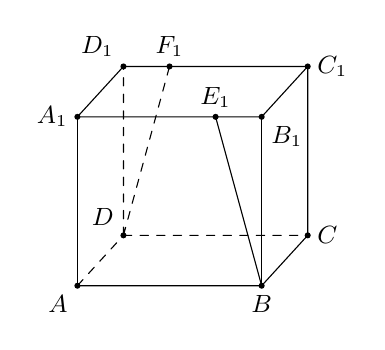
\begin{tikzpicture}[x=.78cm,y=.78cm,font=\small,line cap=round,line join=round]
  \coordinate (A) at (0,0);
  \coordinate (B) at (3,0);
  \coordinate (C) at (3.75,.82);
  \coordinate (D) at (.75,.82);
  \coordinate (Aone) at (0,2.75);
  \coordinate (Bone) at (3,2.75);
  \coordinate (Cone) at (3.75,3.57);
  \coordinate (Done) at (.75,3.57);
  \coordinate (Eone) at (2.25,2.75);
  \coordinate (Fone) at (1.5,3.57);

  % Visible and hidden cube edges follow the source perspective drawing.
  \draw (A)--(B)--(C)--(Cone)--(Bone)--(Aone)--(Done)--(Cone);
  \draw (A)--(Aone) (B)--(Bone) (Done)--(Fone);
  \draw[dashed] (A)--(D) (D)--(C) (D)--(Done) (D)--(Fone);
  % The two lines whose angle is asked for.
  \draw (B)--(Eone);

  \fill (A) circle (1.1pt) (B) circle (1.1pt) (C) circle (1.1pt) (D) circle (1.1pt)
        (Aone) circle (1.1pt) (Bone) circle (1.1pt) (Cone) circle (1.1pt) (Done) circle (1.1pt)
        (Eone) circle (1.1pt) (Fone) circle (1.1pt);
  \node[below left] at (A) {$A$};
  \node[below] at (B) {$B$};
  \node[right] at (C) {$C$};
  \node[above left] at (D) {$D$};
  \node[left] at (Aone) {$A_1$};
  \node[below right] at (Bone) {$B_1$};
  \node[right] at (Cone) {$C_1$};
  \node[above left] at (Done) {$D_1$};
  \node[above] at (Eone) {$E_1$};
  \node[above] at (Fone) {$F_1$};
\end{tikzpicture}
\end{center}
\nopagebreak[4]
（A）$\dfrac{15}{17}$　　（B）$\dfrac12$　　（C）$\dfrac8{17}$　　（D）$\dfrac{\sqrt3}{2}$

\Needspace{4\baselineskip}
\textbf{解析}

设棱长 $1$，取坐标 $A(0,0,0)$、$B(1,0,0)$、$D(0,1,0)$、$A_1(0,0,1)$，

以及 $B_1(1,0,1)$、$D_1(0,1,1)$、$C_1(1,1,1)$。

\Needspace{5\baselineskip}
由 $B_1E_1=\dfrac{A_1B_1}{4}$ 得 $E_1=\left(\dfrac34,0,1\right)$；由 $D_1F_1=\dfrac{D_1C_1}{4}$ 得 $F_1=\left(\dfrac14,1,1\right)$。于是
\nopagebreak[4]
\[\overrightarrow{BE_1}=\left(-\dfrac14,0,1\right),\qquad \overrightarrow{DF_1}=\left(\dfrac14,0,1\right).\]
点积 $=-\dfrac1{16}+1=\dfrac{15}{16}$，两向量模均为 $\sqrt{\dfrac1{16}+1}=\dfrac{\sqrt{17}}{4}$，故夹角余弦为 $\dfrac{15/16}{17/16}=\dfrac{15}{17}$。

\gkanswer{答案：A。}

\end{answer}
\begin{answer}
\gksolhead{11}{}

\textbf{题目}：

已知 $y=\log_a(2-x)$ 是 $x$ 的增函数，则 $a$ 的取值范围是\mbox{（　　）}。

（A）$(0,2)$　　（B）$(0,1)$　　（C）$(1,2)$　　（D）$(2,+\infty)$

\Needspace{4\baselineskip}
\textbf{解析}

令 $u=2-x$，它在 $\mathbb R$ 上关于 $x$ 递减。复合函数 $y=\log_a u$ 关于 $x$ 递增，等价于 $\log_a u$ 关于 $u$ 递减，故 $0<a<1$，即 $a\in(0,1)$。

\gkanswer{答案：B。}

\end{answer}
\begin{answer}
\gksolhead{12}{}

\textbf{题目}：

在 $(1-x^3)(1+x)^{10}$ 的展开式中，$x^5$ 的系数是\mbox{（　　）}。

（A）$-297$　　（B）$-252$　　（C）$297$　　（D）$207$

\Needspace{4\baselineskip}
\textbf{解析}

\Needspace{5\baselineskip}
$(1-x^3)(1+x)^{10}$ 中 $x^5$ 的系数为 $(1+x)^{10}$ 中 $x^5$ 的系数减去 $x^2$ 的系数：
\nopagebreak[4]
\[\binom{10}{5}-\binom{10}{2}=252-45=207.\]

\gkanswer{答案：D。}

\end{answer}
\begin{answer}
\gksolhead{13}{}

\textbf{题目}：

已知直线 $l\perp$ 平面 $\alpha$，直线 $m\subset$ 平面 $\beta$，有下面四个命题：

① $\alpha\parallel\beta\Rightarrow l\perp m$；　　② $\alpha\perp\beta\Rightarrow l\parallel m$；

③ $l\parallel m\Rightarrow\alpha\perp\beta$；　　④ $l\perp m\Rightarrow\alpha\parallel\beta$。

其中正确的两个命题是\mbox{（　　）}。

（A）①与②　　（B）③与④　　（C）②与④　　（D）①与③

\Needspace{4\baselineskip}
\textbf{解析}

\begin{itemize}
\item ① $\alpha\parallel\beta$ 且 $l\perp\alpha$ 得 $l\perp\beta$；又 $m\subset\beta$，故 $l\perp m$。正确。
\item ② 反例：取 $\alpha$ 为水平面、$l$ 为竖直直线，$\beta$ 为竖直平面，$m$ 为 $\beta$ 内一条水平直线，则 $l\perp m$ 而不平行。错误。
\item ③ $l\parallel m$ 且 $l\perp\alpha$ 得 $m\perp\alpha$；又 $m\subset\beta$，故 $\beta\perp\alpha$。正确。
\item ④ 反例：$l$ 为竖直直线，$m$ 为 $\beta$ 内一条与 $l$ 垂直的水平直线，此时 $\beta$ 可绕 $m$ 转动而不必与 $\alpha$ 平行。错误。
\end{itemize}

故正确的为①与③，选 (D)。

\gkanswer{答案：D。}

\end{answer}
\begin{answer}
\gksolhead{14}{}

\textbf{题目}：

\Needspace{5\baselineskip}
等差数列 $\{a_n\},\{b_n\}$ 的前 $n$ 项和分别为 $S_n$ 与 $T_n$，若
\nopagebreak[4]
\[
\frac{S_n}{T_n}=\frac{2n}{3n+1},
\]
则 $\displaystyle\lim_{n\to\infty}\frac{a_n}{b_n}$ 等于\mbox{（　　）}。

（A）$1$　　（B）$\dfrac{\sqrt6}{3}$　　（C）$\dfrac23$　　（D）$\dfrac49$

\Needspace{4\baselineskip}
\textbf{解析}

\Needspace{5\baselineskip}
等差数列中 $S_{2n-1}=(2n-1)a_n$，$T_{2n-1}=(2n-1)b_n$，故
\nopagebreak[4]
\[\frac{a_n}{b_n}=\frac{S_{2n-1}}{T_{2n-1}}=\frac{2(2n-1)}{3(2n-1)+1}=\frac{4n-2}{6n-2}\ \longrightarrow\ \frac23\quad(n\to\infty).\]

\gkanswer{答案：C。}

\end{answer}
\begin{answer}
\gksolhead{15}{}

\textbf{题目}：

用 $1,2,3,4,5$ 这五个数字组成没有重复数字的三位数，其中偶数共有\mbox{（　　）}。

（A）24个　　（B）30个　　（C）40个　　（D）50个

\Needspace{4\baselineskip}
\textbf{解析}

三位数为偶数须个位为 $2$ 或 $4$，共 $2$ 种选法；百位、十位从剩余 $4$ 个数字中任取两个排列，有 $4\times3=12$ 种。故共 $2\times12=24$ 个。

\gkanswer{答案：A。}

\end{answer}
\begin{answer}
\gksolhead{16}{}

\textbf{题目}：

方程 $\log_2(x+1)^2+\log_4(x+1)=5$ 的解是\underline{\qquad\qquad}。

\Needspace{4\baselineskip}
\textbf{解析}

\Needspace{5\baselineskip}
定义域要求 $x+1>0$，即 $x>-1$。此时
\nopagebreak[4]
\[\log_2(x+1)^2=\log_2\bigl[(x+1)^2\bigr]=2\log_2(x+1),\qquad \log_4(x+1)=\frac12\log_2(x+1).\]
令 $y=\log_2(x+1)$，方程化为 $2y+\dfrac y2=5$，得 $y=2$，于是 $x+1=4$，$x=3$。

\gkanswer{答案：$x=3$。}

\end{answer}
\begin{answer}
\gksolhead{17}{}

\textbf{题目}：

已知圆台上、下底面圆周都在球面上，且下底面过球心，母线与底面所成的角为 $\dfrac\pi3$，则圆台的体积与球体积之比为\underline{\qquad\qquad}。

\Needspace{4\baselineskip}
\textbf{解析}

\Needspace{5\baselineskip}
设球半径为 $R$。下底面所在平面过球心，故下底面圆是大圆，半径 $R$。设上底面半径为 $r$、圆台高为 $h$，则上底面圆在球上：
\nopagebreak[4]
\[r^2+h^2=R^2.\]
\Needspace{5\baselineskip}
母线与底面所成角为 $\dfrac\pi3$，其水平投影长为 $R-r$，故
\nopagebreak[4]
\[h=(R-r)\tan\frac\pi3=\sqrt3\,(R-r).\]
联立得 $r^2+3(R-r)^2=R^2$，即 $2r^2-3Rr+R^2=0$，解得 $r=\dfrac R2$（$r=R$ 使 $h=0$，退化舍去），从而 $h=\dfrac{\sqrt3}{2}R$。
\Needspace{5\baselineskip}
圆台体积
\nopagebreak[4]
\[V_{\text{\text{台}}}=\frac{\pi h}{3}(R^2+Rr+r^2)=\frac{\pi}{3}\cdot\frac{\sqrt3 R}{2}\cdot\frac{7R^2}{4}=\frac{7\sqrt3}{24}\pi R^3,\]
\Needspace{5\baselineskip}
球体积 $V_{\text{\text{球}}}=\dfrac43\pi R^3$，故体积比为
\nopagebreak[4]
\[\frac{V_{\text{\text{台}}}}{V_{\text{\text{球}}}}=\frac{7\sqrt3/24}{4/3}=\frac{7\sqrt3}{32}.\]

\gkanswer{答案：$\dfrac{7\sqrt3}{32}$。}

\end{answer}
\begin{answer}
\gksolhead{18}{}

\textbf{题目}：

函数 $y=\cos x+\cos\left(x+\dfrac\pi3\right)$ 的最大值是\underline{\qquad\qquad}。

\Needspace{4\baselineskip}
\textbf{解析}

\Needspace{5\baselineskip}
由和差化积
\nopagebreak[4]
\[\cos x+\cos\left(x+\frac\pi3\right)=2\cos\left(x+\frac\pi6\right)\cos\frac\pi6=\sqrt3\cos\left(x+\frac\pi6\right),\]
故最大值为 $\sqrt3$（当 $x+\dfrac\pi6=2k\pi$ 时取到）。

\gkanswer{答案：$\sqrt3$。}

\end{answer}
\begin{answer}
\gksolhead{19}{}

\textbf{题目}：

若直线 $l$ 过抛物线 $y^2=4(x+1)$ 的焦点，并且与 $x$ 轴垂直，则 $l$ 被抛物线截得的线段长为\underline{\qquad\qquad}。

\Needspace{4\baselineskip}
\textbf{解析}

抛物线 $y^2=4(x+1)$ 的顶点为 $(-1,0)$，由 $y^2=4a(x+1)$ 得 $a=1$，焦点为 $(-1+1,0)=(0,0)$。过焦点且与 $x$ 轴垂直的直线为 $x=0$。代入抛物线：$y^2=4$，即 $y=\pm2$。所截线段端点为 $(0,2),(0,-2)$，长为 $4$。

\gkanswer{答案：$4$。}

\end{answer}
\begin{answer}
\gksolhead{20}{}

\textbf{题目}：

四个不同的小球放入编号为 $1,2,3,4$ 的四个盒中，则恰有一个空盒的放法共有\underline{\qquad\qquad}种。（用数字作答）

\Needspace{4\baselineskip}
\textbf{解析}

\Needspace{5\baselineskip}
恰有一个空盒，先选出空盒，有 $4$ 种；再把 $4$ 个不同的小球放入其余 $3$ 个盒且每盒不空，即把球分成 $2,1,1$ 三组：选 $2$ 球成组有 $\binom42=6$ 种，三组分配到 $3$ 个盒有 $3!=6$ 种。故总数为
\nopagebreak[4]
\[4\times\binom42\times3!=4\times6\times6=144.\]

\gkanswer{答案：$144$。}

\end{answer}
\begin{answer}
\gksolhead{21}{}

\textbf{题目}：

\Needspace{5\baselineskip}
解方程
\nopagebreak[4]
\[
3^{x+2}-3^{2-x}=80
\]

\Needspace{4\baselineskip}
\textbf{解析}

\Needspace{5\baselineskip}
令 $t=3^x>0$，则 $3^{x+2}=9t$，$3^{2-x}=\dfrac9t$。方程化为
\nopagebreak[4]
\[9t-\frac9t=80\iff 9t^2-80t-9=0,\]
解得 $t=\dfrac{80\pm\sqrt{6400+324}}{18}=\dfrac{80\pm82}{18}$，即 $t=9$ 或 $t=-\dfrac19$（负值舍去）。由 $3^x=9$ 得 $x=2$。

\gkanswer{答案：$x=2$。}

\end{answer}
\begin{answer}
\gksolhead{22}{}

\textbf{题目}：

设复数 $z=\cos\theta+i\sin\theta$，$\theta\in(\pi,2\pi)$，求复数 $z^2+z$ 的模和辐角。

\Needspace{4\baselineskip}
\textbf{解析}

\Needspace{5\baselineskip}
由和差化积
\nopagebreak[4]
\[z^2+z=(\cos2\theta+\cos\theta)+i(\sin2\theta+\sin\theta)=2\cos\frac\theta2\left(\cos\frac{3\theta}{2}+i\sin\frac{3\theta}{2}\right).\]
\Needspace{5\baselineskip}
因 $\theta\in(\pi,2\pi)$，有 $\dfrac\theta2\in\left(\dfrac\pi2,\pi\right)$，故 $\cos\dfrac\theta2<0$。于是
\nopagebreak[4]
\[|z^2+z|=\left|2\cos\frac\theta2\right|=-2\cos\frac\theta2,\]
\Needspace{5\baselineskip}
且 $z^2+z$ 的方向与 $e^{i3\theta/2}$ 相反，故
\nopagebreak[4]
\[\arg(z^2+z)=\frac{3\theta}{2}+\pi+2k\pi=\frac{3\theta}{2}-\pi+2k\pi\quad(k\in\mathbb Z).\]
又 $\dfrac{3\theta}{2}-\pi\in\left(\dfrac\pi2,2\pi\right)\subset[0,2\pi)$，可作为辐角主值。

\gkanswer{答案：$|z^2+z|=-2\cos\dfrac\theta2$（即 $2\left|\cos\dfrac\theta2\right|$）；辐角主值为 $\dfrac{3\theta}{2}-\pi$。}

\end{answer}
\begin{answer}
\gksolhead{23}{}

\textbf{题目}：

\Needspace{5\baselineskip}
设 $\{a_n\}$ 是由正数组成的等比数列，$S_n$ 是其前 $n$ 项和，证明：
\nopagebreak[4]
\[
\frac{\log_{0.5}S_n+\log_{0.5}S_{n+2}}{2}>\log_{0.5}S_{n+1}
\]

\Needspace{4\baselineskip}
\textbf{解析}

\Needspace{5\baselineskip}
设 $\{a_n\}$ 首项 $a_1>0$、公比 $q>0$，则各项为正，$S_n>0$。因 $\log_{0.5}$ 在 $(0,+\infty)$ 上递减，原不等式等价于证明
\nopagebreak[4]
\[S_nS_{n+2}<S_{n+1}^2.\]
\Needspace{5\baselineskip}
计算
\nopagebreak[4]
\[S_{n+1}^2-S_nS_{n+2}=S_{n+1}^2-S_n(S_{n+1}+a_{n+2})=a_{n+1}S_{n+1}-a_{n+2}S_n.\]
\Needspace{5\baselineskip}
由 $a_{n+2}=qa_{n+1}$，得
\nopagebreak[4]
\[S_{n+1}^2-S_nS_{n+2}=a_{n+1}(S_{n+1}-qS_n).\]
\Needspace{5\baselineskip}
又 $S_{n+1}=a_1+qS_n$，故 $S_{n+1}-qS_n=a_1$，从而
\nopagebreak[4]
\[S_{n+1}^2-S_nS_{n+2}=a_1a_{n+1}>0.\]
\Needspace{5\baselineskip}
于是 $S_{n+1}>\sqrt{S_nS_{n+2}}$，由 $\log_{0.5}$ 递减得
\nopagebreak[4]
\[\log_{0.5}S_{n+1}<\log_{0.5}\sqrt{S_nS_{n+2}}=\frac{\log_{0.5}S_n+\log_{0.5}S_{n+2}}{2}.\]

\gkanswer{答案：不等式对任意正整数 $n$ 成立（证明见解析）。}

\end{answer}
\begin{answer}
\gksolhead{24}{}

\textbf{题目}：

如图，圆柱的轴截面 $ABCD$ 是正方形，点 $E$ 在底面的圆周上，$AF\perp DE$，$F$ 是垂足。
\nopagebreak[4]
\begin{center}% 固定来源PDF印刷页52第24题圆柱、轴截面和垂足的矢量示意重绘。
% 使用斜投影表达拓扑关系；圆柱比例不代表题设精确度量。
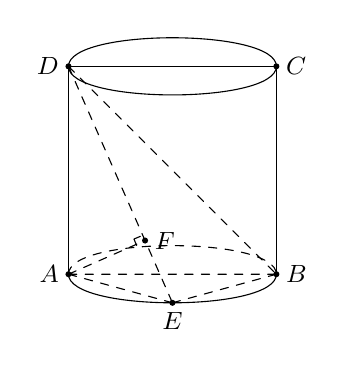
\begin{tikzpicture}[x=.88cm,y=.88cm,font=\small,line cap=round,line join=round]
  \coordinate (A) at (-1.5,0);
  \coordinate (B) at (1.5,0);
  \coordinate (C) at (1.5,3);
  \coordinate (D) at (-1.5,3);
  \coordinate (E) at (0,-.4125);
  \coordinate (F) at (-.395,.486);

  % Cylinder sides and top circular rim.
  \draw (A)--(D) (B)--(C);
  \draw (D) .. controls (-1.5,3.55) and (1.5,3.55) .. (C);
  \draw (D)--(C);
  \draw (D) .. controls (-1.5,2.45) and (1.5,2.45) .. (C);
  % The rear half of the lower rim is hidden; the near half is visible.
  \draw[dashed] (A) .. controls (-1.5,.55) and (1.5,.55) .. (B);
  \draw (A) .. controls (-1.5,-.55) and (1.5,-.55) .. (B);

  % Axial-section diagonal, the perpendicular construction and its foot.
  \draw[dashed] (A)--(B) (D)--(B) (D)--(E) (A)--(F) (A)--(E) (B)--(E);
  % Small right-angle marker at F, fitted to the schematic projections of AF and DE.
  \draw (-.5165,.4155)--(-.5554,.5076)--(-.4633,.5465);
  \fill (A) circle (1.1pt) (B) circle (1.1pt) (C) circle (1.1pt)
        (D) circle (1.1pt) (E) circle (1.1pt) (F) circle (1.1pt);
  \node[left] at (A) {$A$};
  \node[right] at (B) {$B$};
  \node[right] at (C) {$C$};
  \node[left] at (D) {$D$};
  \node[below] at (E) {$E$};
  \node[right] at (F) {$F$};
\end{tikzpicture}
\end{center}
\nopagebreak[4]
（1）求证：$AF\perp DB$；

（2）如果圆柱与三棱锥 $D-ABE$ 的体积的比等于 $3\pi$，求点 $E$ 到截面 $ABCD$ 的距离。

\Needspace{4\baselineskip}
\textbf{解析}

（1）$AB$ 为底面圆直径、$E$ 在底面圆周上，故 $BE\perp AE$（直径所对圆周角为直角）。$AD$ 为母线，垂直于底面，故 $AD\perp BE$。$AE$ 与 $AD$ 是平面 $ADE$ 内两条相交直线，于是 $BE\perp$ 平面 $ADE$；又 $AF\subset$ 平面 $ADE$，故 $BE\perp AF$。题设 $AF\perp DE$，而 $BE$ 与 $DE$ 是平面 $BDE$ 内两条相交直线，故 $AF\perp$ 平面 $BDE$。因 $DB\subset$ 平面 $BDE$，得 $AF\perp DB$。

\Needspace{5\baselineskip}
（2）设底面半径为 $r$，圆柱高为 $h$。轴截面为正方形，故 $h=AB=2r$。设点 $E$ 到底面直线 $AB$ 的距离为 $d$，则
\nopagebreak[4]
\[S_{\triangle ABE}=\frac12\cdot2r\cdot d=rd,\qquad V_{D-ABE}=\frac13\cdot rd\cdot2r=\frac23r^2d.\]
\Needspace{5\baselineskip}
圆柱体积为 $V_{\mathrm{\text{柱}}}=\pi r^2h=2\pi r^3$，由体积比得
\nopagebreak[4]
\[\frac{V_{\mathrm{\text{柱}}}}{V_{D-ABE}}=\frac{2\pi r^3}{\frac23r^2d}=\frac{3\pi r}{d}=3\pi,\]
因此 $d=r$。截面 $ABCD$ 垂直于底面，交线为 $AB$，故 $E$ 到截面的距离即为 $d$，等于底面半径。该值可达到（底面半圆弧中点），且长度量纲一致；来源未给半径数值，保留以 $r$ 表示的结果。

\gkanswer{答案：（1）$AF\perp DB$；（2）点 $E$ 到截面 $ABCD$ 的距离等于圆柱底面半径。}

\end{answer}
\begin{answer}
\gksolhead{25}{}

\textbf{题目}：

\Needspace{5\baselineskip}
某地为促进淡水鱼养殖业的发展，将价格控制在适当范围内，决定对淡水鱼养殖提供政府补贴。设淡水鱼的市场价格为 $x$ 元/千克，政府补贴为 $t$ 元/千克。根据市场调查，当 $8\le x\le14$ 时，淡水鱼的市场日供应量 $P$ 千克与市场日需求量 $Q$ 千克近似满足关系：
\nopagebreak[4]
\[
P=1000(x+t-8)\quad(x\ge8,\ t\ge0),\qquad
Q=500\sqrt{40-(x-8)^2}\quad(8\le x\le14)
\]
当 $P=Q$ 时市场价格称为市场平衡价格。

（1）将市场平衡价格表示为政府补贴的函数，并求出函数的定义域；

（2）为使市场平衡价格不高于每千克10元，政府补贴至少为每千克多少元？

\Needspace{4\baselineskip}
\textbf{解析}

\Needspace{5\baselineskip}
（1）由 $P=Q$ 得
\nopagebreak[4]
\[1000(x+t-8)=500\sqrt{40-(x-8)^2}\iff 2(x+t-8)=\sqrt{40-(x-8)^2}.\]
\Needspace{5\baselineskip}
两边非负，平方不失解。令 $u=x-8\in[0,6]$，得
\nopagebreak[4]
\[4(u+t)^2=40-u^2\iff 5u^2+8tu+4t^2-40=0,\]
\Needspace{5\baselineskip}
解得
\nopagebreak[4]
\[u=\frac{-8t\pm\sqrt{64t^2-20(4t^2-40)}}{10}=\frac{-4t\pm2\sqrt{50-t^2}}{5}.\]
\Needspace{5\baselineskip}
因 $u\ge0$，只取加号：$u=\dfrac{2\sqrt{50-t^2}-4t}{5}$。其有意义的条件为 $50-t^2\ge0$ 且 $u\ge0$；后者等价于 $\sqrt{50-t^2}\ge2t\iff 50-t^2\ge4t^2\iff t^2\le10$。综上 $t\in[0,\sqrt{10}]$，且此时 $x=8+u\in[8,\,8+2\sqrt2]\subset[8,14]$。故
\nopagebreak[4]
\[x=8+\frac{2\sqrt{50-t^2}-4t}{5},\qquad t\in[0,\sqrt{10}].\]

\Needspace{5\baselineskip}
（2）由第一问，
\nopagebreak[4]
\[x'(t)=-\frac{2t}{5\sqrt{50-t^2}}-\frac45<0\qquad(0\le t\le\sqrt{10}),\]
故平衡价格随补贴严格下降。令 $x=10$，由原平衡式得 $2(10+t-8)=\sqrt{40-(10-8)^2}=6$，解得 $t=1$。于是 $x\le10$ 等价于 $t\ge1$（并满足第一问定义域），最低补贴为每千克 $1$ 元。代回 $t=1,x=10$，供应与需求同为 $3000$ 千克，单位及边界均相符。

\gkanswer{答案：（1）$x=8+\dfrac{2\sqrt{50-t^2}-4t}{5}$，$t\in[0,\sqrt{10}]$；（2）政府补贴至少为每千克 $1$ 元。}

\end{answer}
\begin{answer}
\gksolhead{26}{}

\textbf{题目}：

\Needspace{5\baselineskip}
已知椭圆
\nopagebreak[4]
\[
\frac{x^2}{24}+\frac{y^2}{16}=1
\]
\Needspace{5\baselineskip}
直线 $l:x=12$。$P$ 是 $l$ 上一点，射线 $OP$ 交椭圆于点 $R$，又点 $Q$ 在 $OP$ 上且满足
\nopagebreak[4]
\[
|OQ|\cdot|OP|=|OR|^2
\]
当点 $P$ 在 $l$ 上移动时，求点 $Q$ 的轨迹方程，并说明轨迹是什么曲线。

\Needspace{4\baselineskip}
\textbf{解析}

\Needspace{5\baselineskip}
设 $P(12,m)$（$m\in\mathbb R$）。射线 $OP$ 上的点可写成 $\lambda(12,m)\ (\lambda\ge0)$。设 $R$ 对应参数 $\lambda$，代入椭圆：
\nopagebreak[4]
\[\frac{(12\lambda)^2}{24}+\frac{(m\lambda)^2}{16}=1\iff \lambda^2\left(6+\frac{m^2}{16}\right)=1,\]
\Needspace{5\baselineskip}
故 $|OR|^2=\lambda^2|OP|^2$。设 $Q=\mu(12,m)\ (\mu>0)$，由 $|OQ|\cdot|OP|=|OR|^2$ 得
\nopagebreak[4]
\[\mu|OP|^2=\lambda^2|OP|^2\iff \mu=\lambda^2=\frac{1}{6+m^2/16}=\frac{16}{96+m^2}.\]
\Needspace{5\baselineskip}
（此时 $0<\mu\le\dfrac16<1$，$Q$ 确实在线段 $OP$ 上。）于是
\nopagebreak[4]
\[x=12\mu=\frac{192}{96+m^2},\qquad y=m\mu=\frac{16m}{96+m^2}.\]
\Needspace{5\baselineskip}
由 $y=\dfrac{mx}{12}$ 得 $m=\dfrac{12y}{x}$；由第一式得 $m^2=\dfrac{192}{x}-96=\dfrac{192-96x}{x}$。代入 $m^2$：
\nopagebreak[4]
\[\frac{144y^2}{x^2}=\frac{192-96x}{x}\Longrightarrow 144y^2=192x-96x^2\Longrightarrow 2x^2+3y^2=4x.\]
\Needspace{5\baselineskip}
又 $x=\dfrac{192}{96+m^2}\in(0,2]$，原点 $(0,0)$ 对应 $m\to\infty$，取不到。配方得
\nopagebreak[4]
\[\frac{(x-1)^2}{1}+\frac{y^2}{2/3}=1,\]
即轨迹为椭圆（半长轴 $1$、半短轴 $\dfrac{\sqrt6}{3}$，长轴沿 $x$ 轴），去掉原点。

\gkanswer{答案：$(x-1)^2+\dfrac32y^2=1$（即 $2x^2+3y^2=4x$），$0<x\le2$，除去原点。}

\end{answer}